%!TEX root = ../template.tex
%%%%%%%%%%%%%%%%%%%%%%%%%%%%%%%%%%%%%%%%%%%%%%%%%%%%%%%%%%%%%%%%%%%%
%% chapter3.tex
%% NOVA thesis document file
%%
%% Chapter with a short latex tutorial and examples
%%%%%%%%%%%%%%%%%%%%%%%%%%%%%%%%%%%%%%%%%%%%%%%%%%%%%%%%%%%%%%%%%%%%

\typeout{NT FILE chapter3.tex}%

%\makeatletter
%\newcommand{\ntifpkgloaded}{%
%  \@ifpackageloaded%
%}
%\makeatother

%Proposta de trabalho

\chapter{Project Description, Time Planning and Previous Work}
\label{cha:projectDescription}


\section{Project Description}
\label{sec:project_description}

For this project, for each foot, an Arduino Nano 33 BLE will be used. These devices have an integrated IMU each that captures acceleration and orientation and they work with BLE %reference BLE.

This project will focus on the use-case of smart insoles for movement analysis and injury prevention in basketball since there aren't many papers about the 
merging of footwork recognition and marginal gains or injury prevention.


The project can be separated in five big goals:

\begin{enumerate}
    \item User Interface - Android Application Development
    \item \item Recognise basic basketball movements/footwork
    \item Recognise intermediate and Advanced basketball movements/footwork
    \item Recognise harmful movements
    \item Identify possible improvements
\end{enumerate}

The methods used in the project are described in \autoref{sec:data_analysis}.

All the different basketball movements analyzed in this project are described in the \Autoref{ssec:other_movements}.

\newpage
\section{Time Planning}
\label{sec:time_planning}

The following \autoref{fig:ganttChart} is the project's ghant chart which outlines the timeline and the milestones of the project, providing a visual representation of the tasks, their durations, 
and dependencies.

\begin{figure}[htbp]
    \centering
    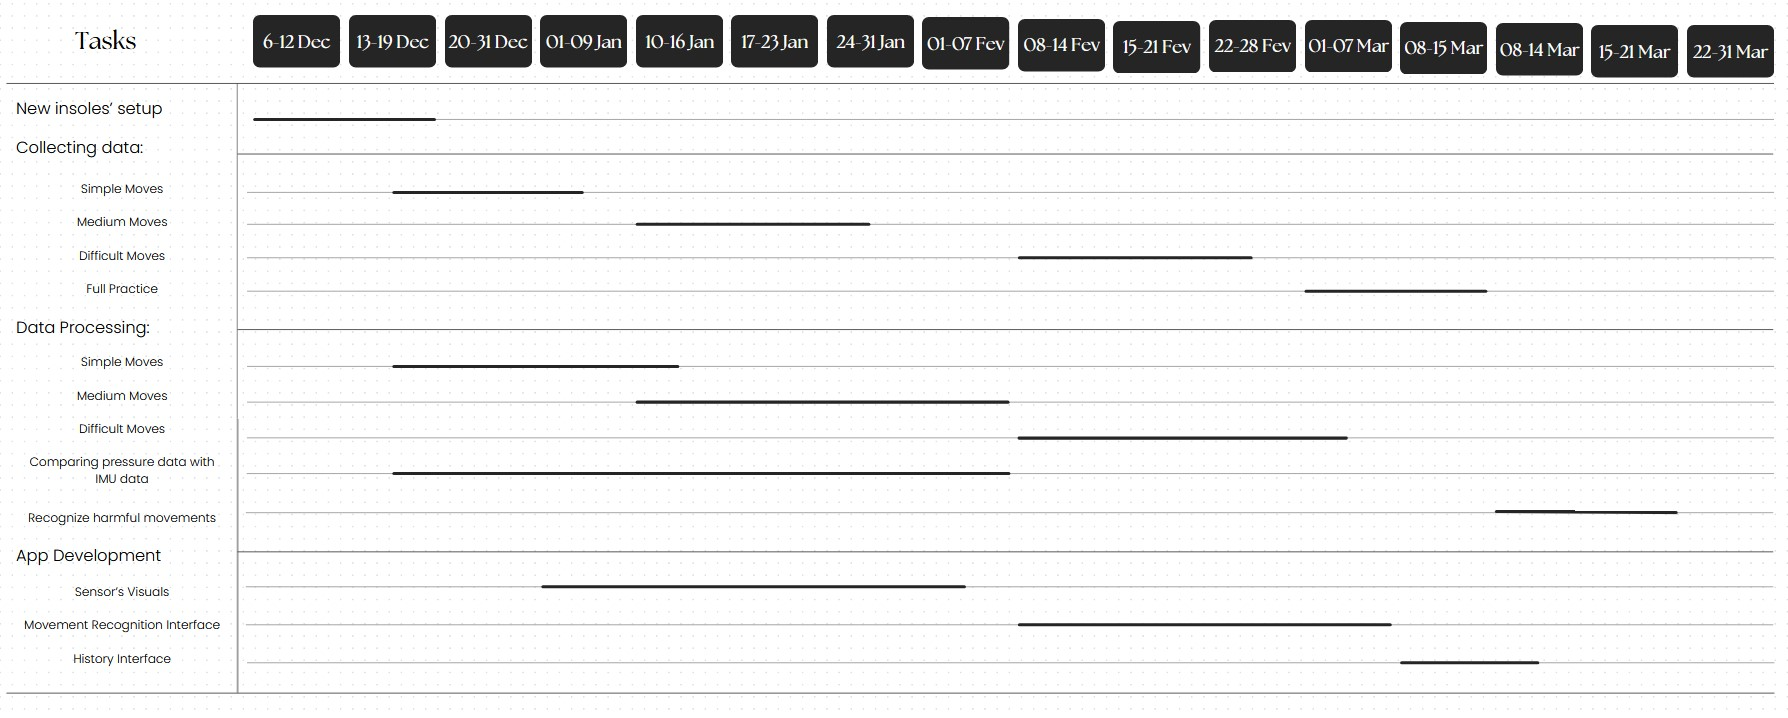
\includegraphics[width=\linewidth]{ganttChart.jpg}
    \caption{Project's Gantt Chart.}
    \label{fig:ganttChart}
\end{figure}

\section{Previous Work}
\label{sec:previous_work}

There have been two other projects based in the last two insole prototypes: 

A Master's Thesis in 2020 that focused in the device's design and and it's use cases for 
diabetic monotoring and back injury's prevention in heavy lifts. An android app that serves as an user's interface for the insoles was also developed~\cite{masterInsole}. 

The other one was a Bachelor Project in 2021 that continued the previous work on heavy lifting focusing on the classification of proper/improper lifts, 
load's weight estimation and visual feedback for the user. Further development was also done in the app~\cite{bachelorInsole}. 

\subsection{Insole Prototype}
\label{ssub:insoleProt}

The insoles have sixteen sensors build with piezoresistive fabric, Polyvinylidene fluoride (PVDF), making the flexible and appropriate for this case. 
As explained before this means that any pressure change on the sensors produces a proportional electrical charge. If the sensors get static there won't be any charge.
They also have temperature sensors integrated since they we're primarily designed for diabetic monotoring but for this project they aren't relevant. They also have an IMU that will 
be useful to difer each movement.

The sensors are distributed in pairs in eight specifically chosen locations to cover the metatarsals, hallux and heel contact points in the plantar plane. 
These are also designed to work broadly with every shape of feet.

\begin{figure}[htbp]
    \centering
    \subbottom[Example of a plantar map\label{fig:plantarMap}]{%
      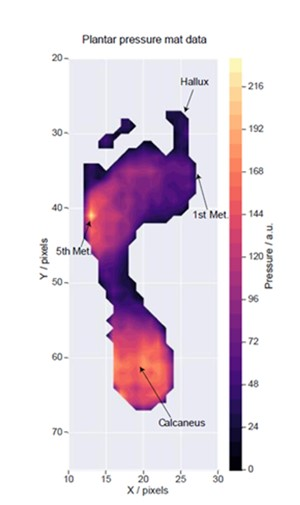
\includegraphics[width=0.35\linewidth]{plantarMap}}%
    \subbottom[Locations of the sensors\label{fig:prototype}]{%
      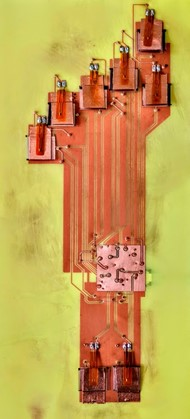
\includegraphics[width=0.25\linewidth]{prototype}}%
    %\caption{}
    \label{fig:insole}
  \end{figure}

The data collected is filtered and converted to reduce packet size. Then it is sent to the movile phone via BLE to use the least amount of energy possible. Afterwards it is sent to the database through WiFi~\cite{masterInsole}.

%\begin{figure}[htbp]
%  \centering
%  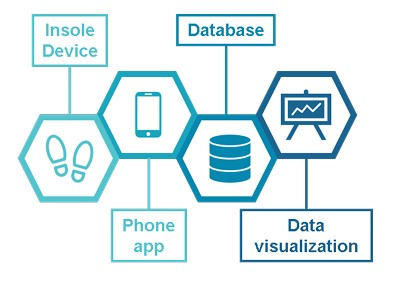
\includegraphics[width=0.9\linewidth]{system.jpg}
%  \caption{System overview~\cite{masterInsole}.}
%  \label{fig:system}
%\end{figure}


% \printbibliography[heading=subbibliography, segment=\therefsegment, title={\bibname\ for chapter~\thechapter}]

